% ------------------------------------------------------------------------------
% TYPO3 Version 10.3 - What's New (French Version)
%
% @license	Creative Commons BY-NC-SA 3.0
% @link		https://typo3.org/help/documentation/whats-new/
% @language	French
% ------------------------------------------------------------------------------

\section{Sécurité et Vie privée}
\begin{frame}[fragile]
	\frametitle{Sécurité et Vie privée}

	\begin{center}\huge{Chapitre 5~:}\end{center}
	\begin{center}\huge{\color{typo3darkgrey}\textbf{Sécurité et Vie privée}}\end{center}

\end{frame}

% ------------------------------------------------------------------------------
% Feature | 90333 | Dashboard

\begin{frame}[fragile]
	\frametitle{Sécurité et Vie privée}
	\framesubtitle{Tableau de bord}

	\begin{itemize}
		\item Les widgets du tableau de bord peuvent contenir des informations sensibles.
		\item Ainsi, nous recommandons la mise en place de permissions basée sur les groupes.
		\item Les utilisateurs backend n'ont accès qu'aux widgets qui leurs sont disponibles.
		\item Les administrateurs possèdent toujours l'accès à tous les widgets.
	\end{itemize}

\end{frame}

% ------------------------------------------------------------------------------
% Feature | 89978 | Introduce Status Report for insecure exception handler settings

\begin{frame}[fragile]
	\frametitle{Sécurité et Vie privée}
	\framesubtitle{Rapport}

	\begin{itemize}
		\item DebugExceptionHandler peut afficher des données sensibles, ce qui
			peut devenir une vulnérabilité de divulgation d'informations.
		\item Une nouvelle entrée de rapport fourni un avertissement aux administrateurs.
	\end{itemize}

	\vspace{0.4cm}
	\textbf{AVERTISSEMENT}, si le contexte est \textbf{development} et la sortie d'erreur est activée~:
	\begin{figure}
		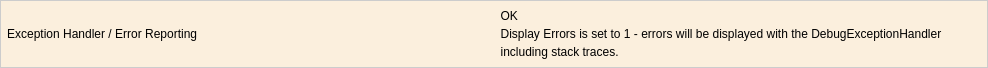
\includegraphics[width=1\linewidth]{SecurityAndPrivacy/89978a-IntroduceStatusReportForInsecureExceptionHandlerSettings.png}
	\end{figure}

	\textbf{ERREUR}, si le contexte est \textbf{production} et la sortie d'erreur est activée~:
	\begin{figure}
		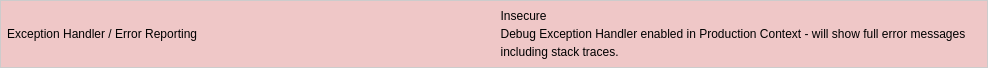
\includegraphics[width=1\linewidth]{SecurityAndPrivacy/89978b-IntroduceStatusReportForInsecureExceptionHandlerSettings.png}
	\end{figure}

\end{frame}

% ------------------------------------------------------------------------------
% Feature | 90351 | Allow TYPO3 to make SameSite cookies configurable

\begin{frame}[fragile]
	\frametitle{Sécurité et Vie privée}
	\framesubtitle{Cookies du même site (1)}

	\begin{itemize}
		\item Pour renforcer la sécurité et vie privée, TYPO3 supporte l'option «~SameSite~»
			pour les cookies gérés par le noyau de TYPO3.
		\item L'attribut est supporté par la majorité des navigateurs modernes et permet aux sites
			de déclarer si les cookies doivent être restreints.
		\item Selon
			\href{https://www.owasp.org/index.php/SameSite}{OWASP}, l'option\newline
			\small
				«~\textit{atténue le risque de fuite d'information inter-sources}~», avec\newline
				«~\textit{des protections contre les attaques par requête forgées inter-sites}~».
			\normalsize

		\item Les configurations valides sont «~\textbf{strict}~», «~\textbf{lax}~», ou \textit{non défini}.
	\end{itemize}

\end{frame}

% ------------------------------------------------------------------------------
% Feature | 90351 | Allow TYPO3 to make SameSite cookies configurable

\begin{frame}[fragile]
	\frametitle{Sécurité et Vie privée}
	\framesubtitle{Cookies du même site (2)}

	\begin{itemize}
		\item TYPO3 défini les configurations suivantes~:

			\begin{itemize}\small
				\item Session d'utilisateur FE~: «~lax~» par défaut
				\item Session d'utilisateur BE~: «~strict~» par défaut
				\item Session de l'outil d'installation~: «~strict~» (non configurable)
				\item Dernier fournisseur d'authentification (BE)~: «~strict~» (non configurable)
			\end{itemize}\normalsize

		\item L'outil d'installation offre une configuration système pour ajuster
			la politique de l'option SameSite, si la configuration par défaut est trop stricte
			(i.e. avec les fournisseurs d'authentification comme OpenID/OAuth).

		\item En savoir plus sur les cookies de même site dans la
			\href{https://tools.ietf.org/html/draft-ietf-httpbis-cookie-same-site-00}{RFC6265} (brouillon).
	\end{itemize}

\end{frame}

% ------------------------------------------------------------------------------
% Feature | 90262 | Add Argon2id to password hash algorithms

\begin{frame}[fragile]
	\frametitle{Sécurité et Vie privée}
	\framesubtitle{Algorithme de hachage des mots de passe}

	\begin{itemize}
		\item L'algorithme de hachage \texttt{Argon2i} («~i~») fut introduit dans TYPO3 v9 LTS.
		\item \texttt{Argon2id} («~id~») est disponible dans TYPO3 si la version de PHP le supporte.
		\item \texttt{Argon2id} est un hybride entre \texttt{Argon2i} et \texttt{Argon2d}
			et est plus résistant contre les attaques par canaux auxiliaires.
		\item \texttt{Argon2id} est habituellement disponible sur les systèmes avec PHP version 7.3 ou ultérieur.
	\end{itemize}

\end{frame}

% ------------------------------------------------------------------------------
